\begin{figure*}
\begin{center}
% \vspace{-6pt}
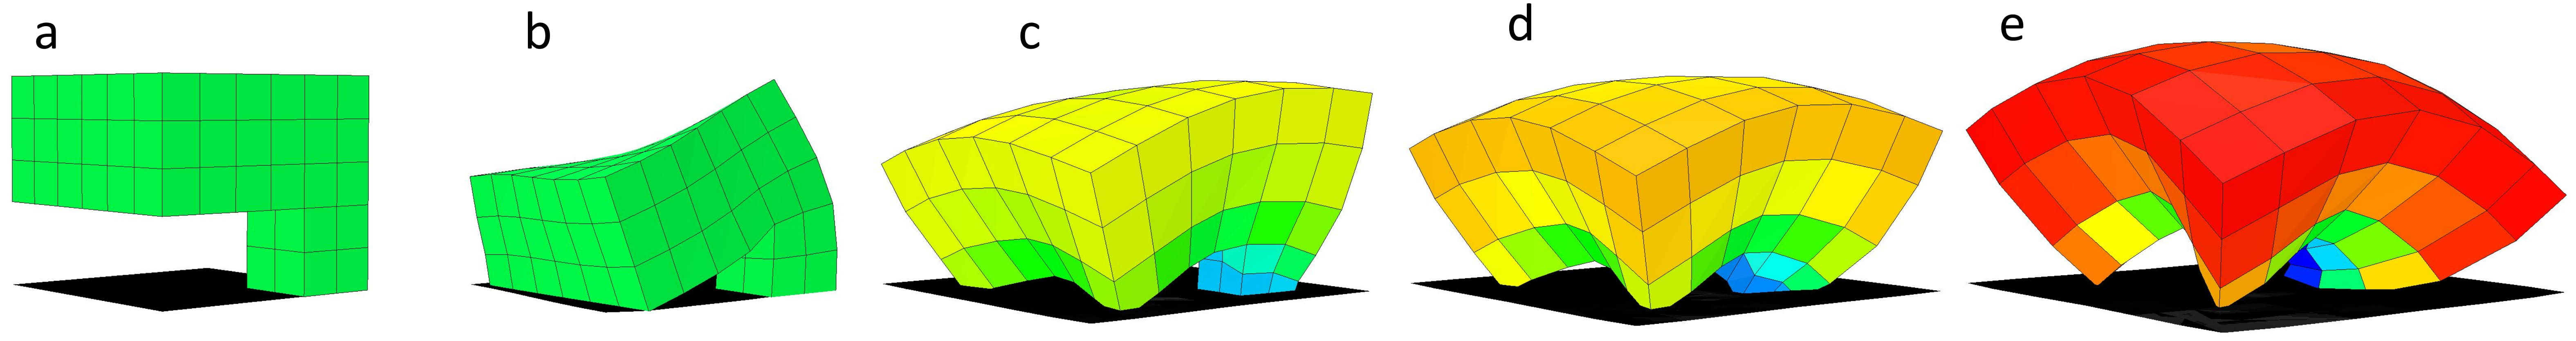
\includegraphics[trim={-40pt 0 0 0},clip,width=\linewidth]{Chapter05/fig/tucker.jpg} \\
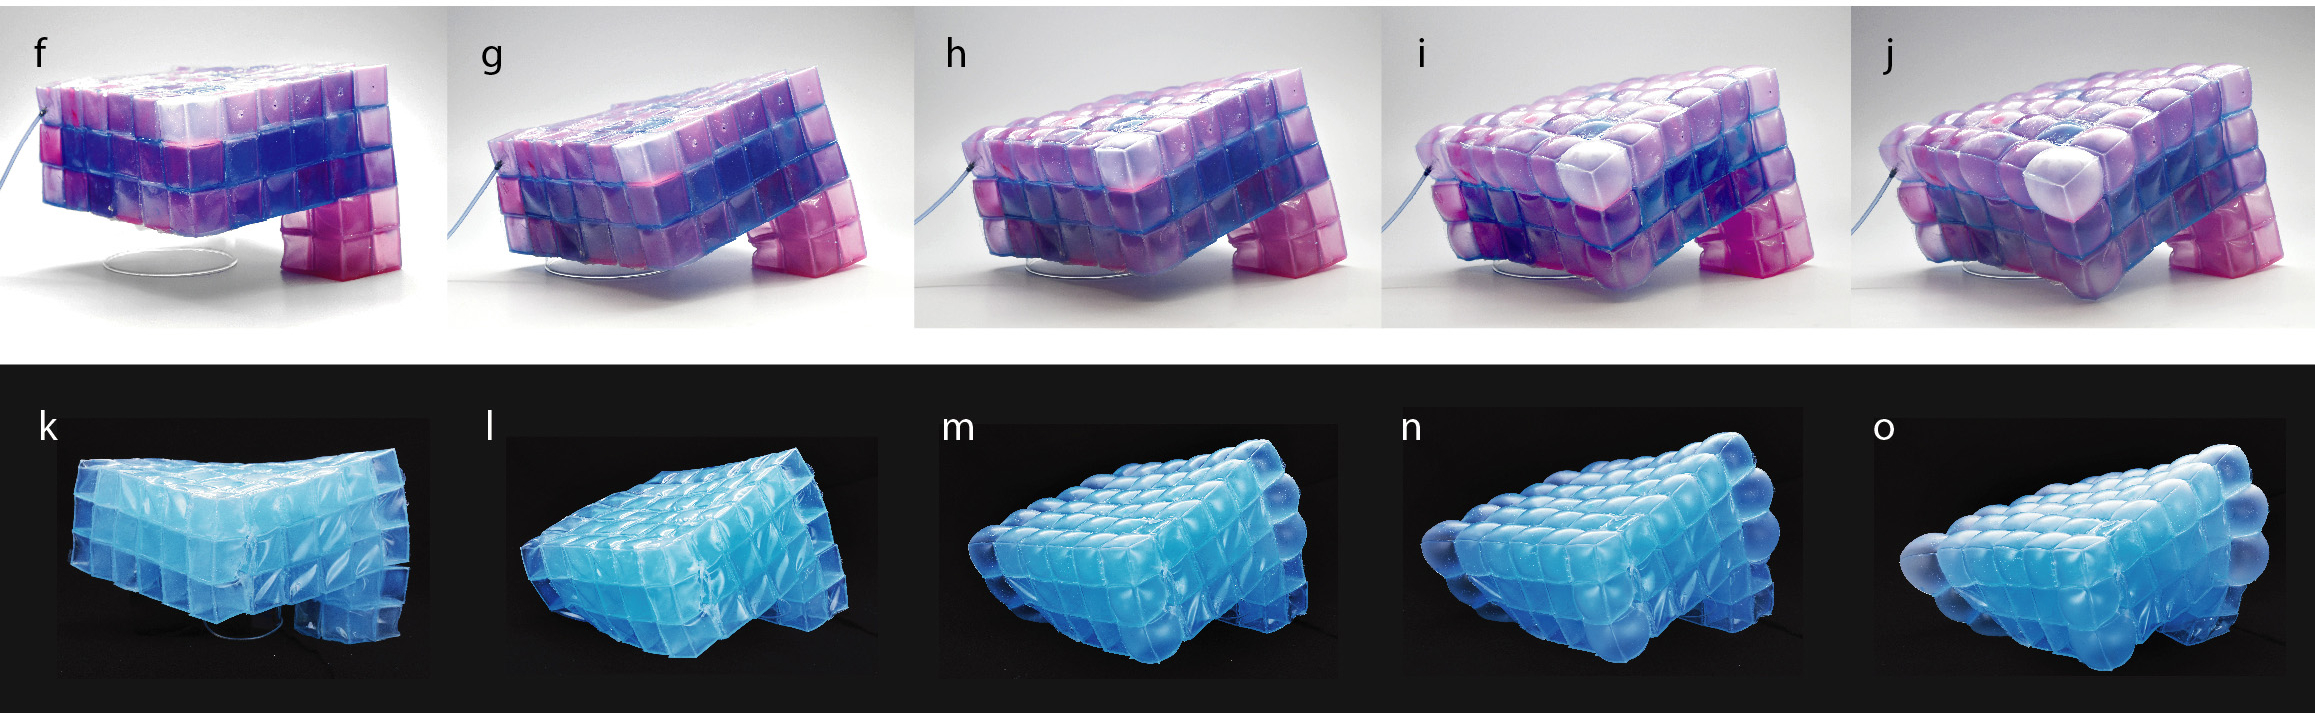
\includegraphics[trim={0 0 0 -5pt},clip,width=\linewidth]{Chapter05/fig/VoxelBotTuckerCropped.jpg}\\
% \vspace{-2pt}
\caption{\label{fig:tucker}After losing three legs to injury (amp.~=~3~legs), the former quadruped is reduced to a monopedal structure~(\textbf{a}), the shape of which was then optimized for locomotion speed, resulting in an expanded spine, the folding-inward of the remnant predamage leg, and the ``regeneration'' of the three missing legs~(\textbf{c-e}).
This simulated strategy was then realized in two implementations using pneumatically-actuated, cubic elastomer bladders. The purple robot~(\textbf{f-j}) consists of two layers of drip-molded silicone; the blue robot~(\textbf{k-o}) consists of a single layer, and is thus less stable but more deformable.
A single air inlet here yields the rudiments of appropriate shape change, but pressure oscillations in this setup did not yield locomotion
(\href{https://youtu.be/A2KTGhCFxK8}{\textcolor{blue}{\textbf{\texttt{youtu.be/A2KTGhCFxK8}}}}).
}
% \vspace{-2em}
\end{center}
\end{figure*}